\documentclass{beamer}
\usepackage{tikz,amsmath,hyperref,graphicx,stackrel,animate,amssymb}
\usetikzlibrary{positioning,shadows,arrows,shapes,calc}
\newcommand{\argmax}{\operatornamewithlimits{argmax}}
\newcommand{\argmin}{\operatornamewithlimits{argmin}}
\newcommand{\average}{\operatornamewithlimits{average}}
\mode<presentation>{\usetheme{Frankfurt}}
\AtBeginSection[]
{
  \begin{frame}<beamer>
    \frametitle{Outline}
    \tableofcontents[currentsection,currentsubsection]
  \end{frame}
}
\title{Lecture 5: Short-Time Fourier Transform and Filterbanks}
\author{Mark Hasegawa-Johnson\\These slides are in the public domain.}
\date{ECE 417: Multimedia Signal Processing, Fall 2020}  
\begin{document}

% Title
\begin{frame}
  \maketitle
\end{frame}

% Title
\begin{frame}
  \tableofcontents
\end{frame}

%%%%%%%%%%%%%%%%%%%%%%%%%%%%%%%%%%%%%%%%%%%%
\section[STFT]{Short-Time Fourier Transform}
\setcounter{subsection}{1}

\begin{frame}
  \frametitle{Spectrogram = $20\log_{10}|\mbox{Short Time Fourier Transform}|$}
  \centerline{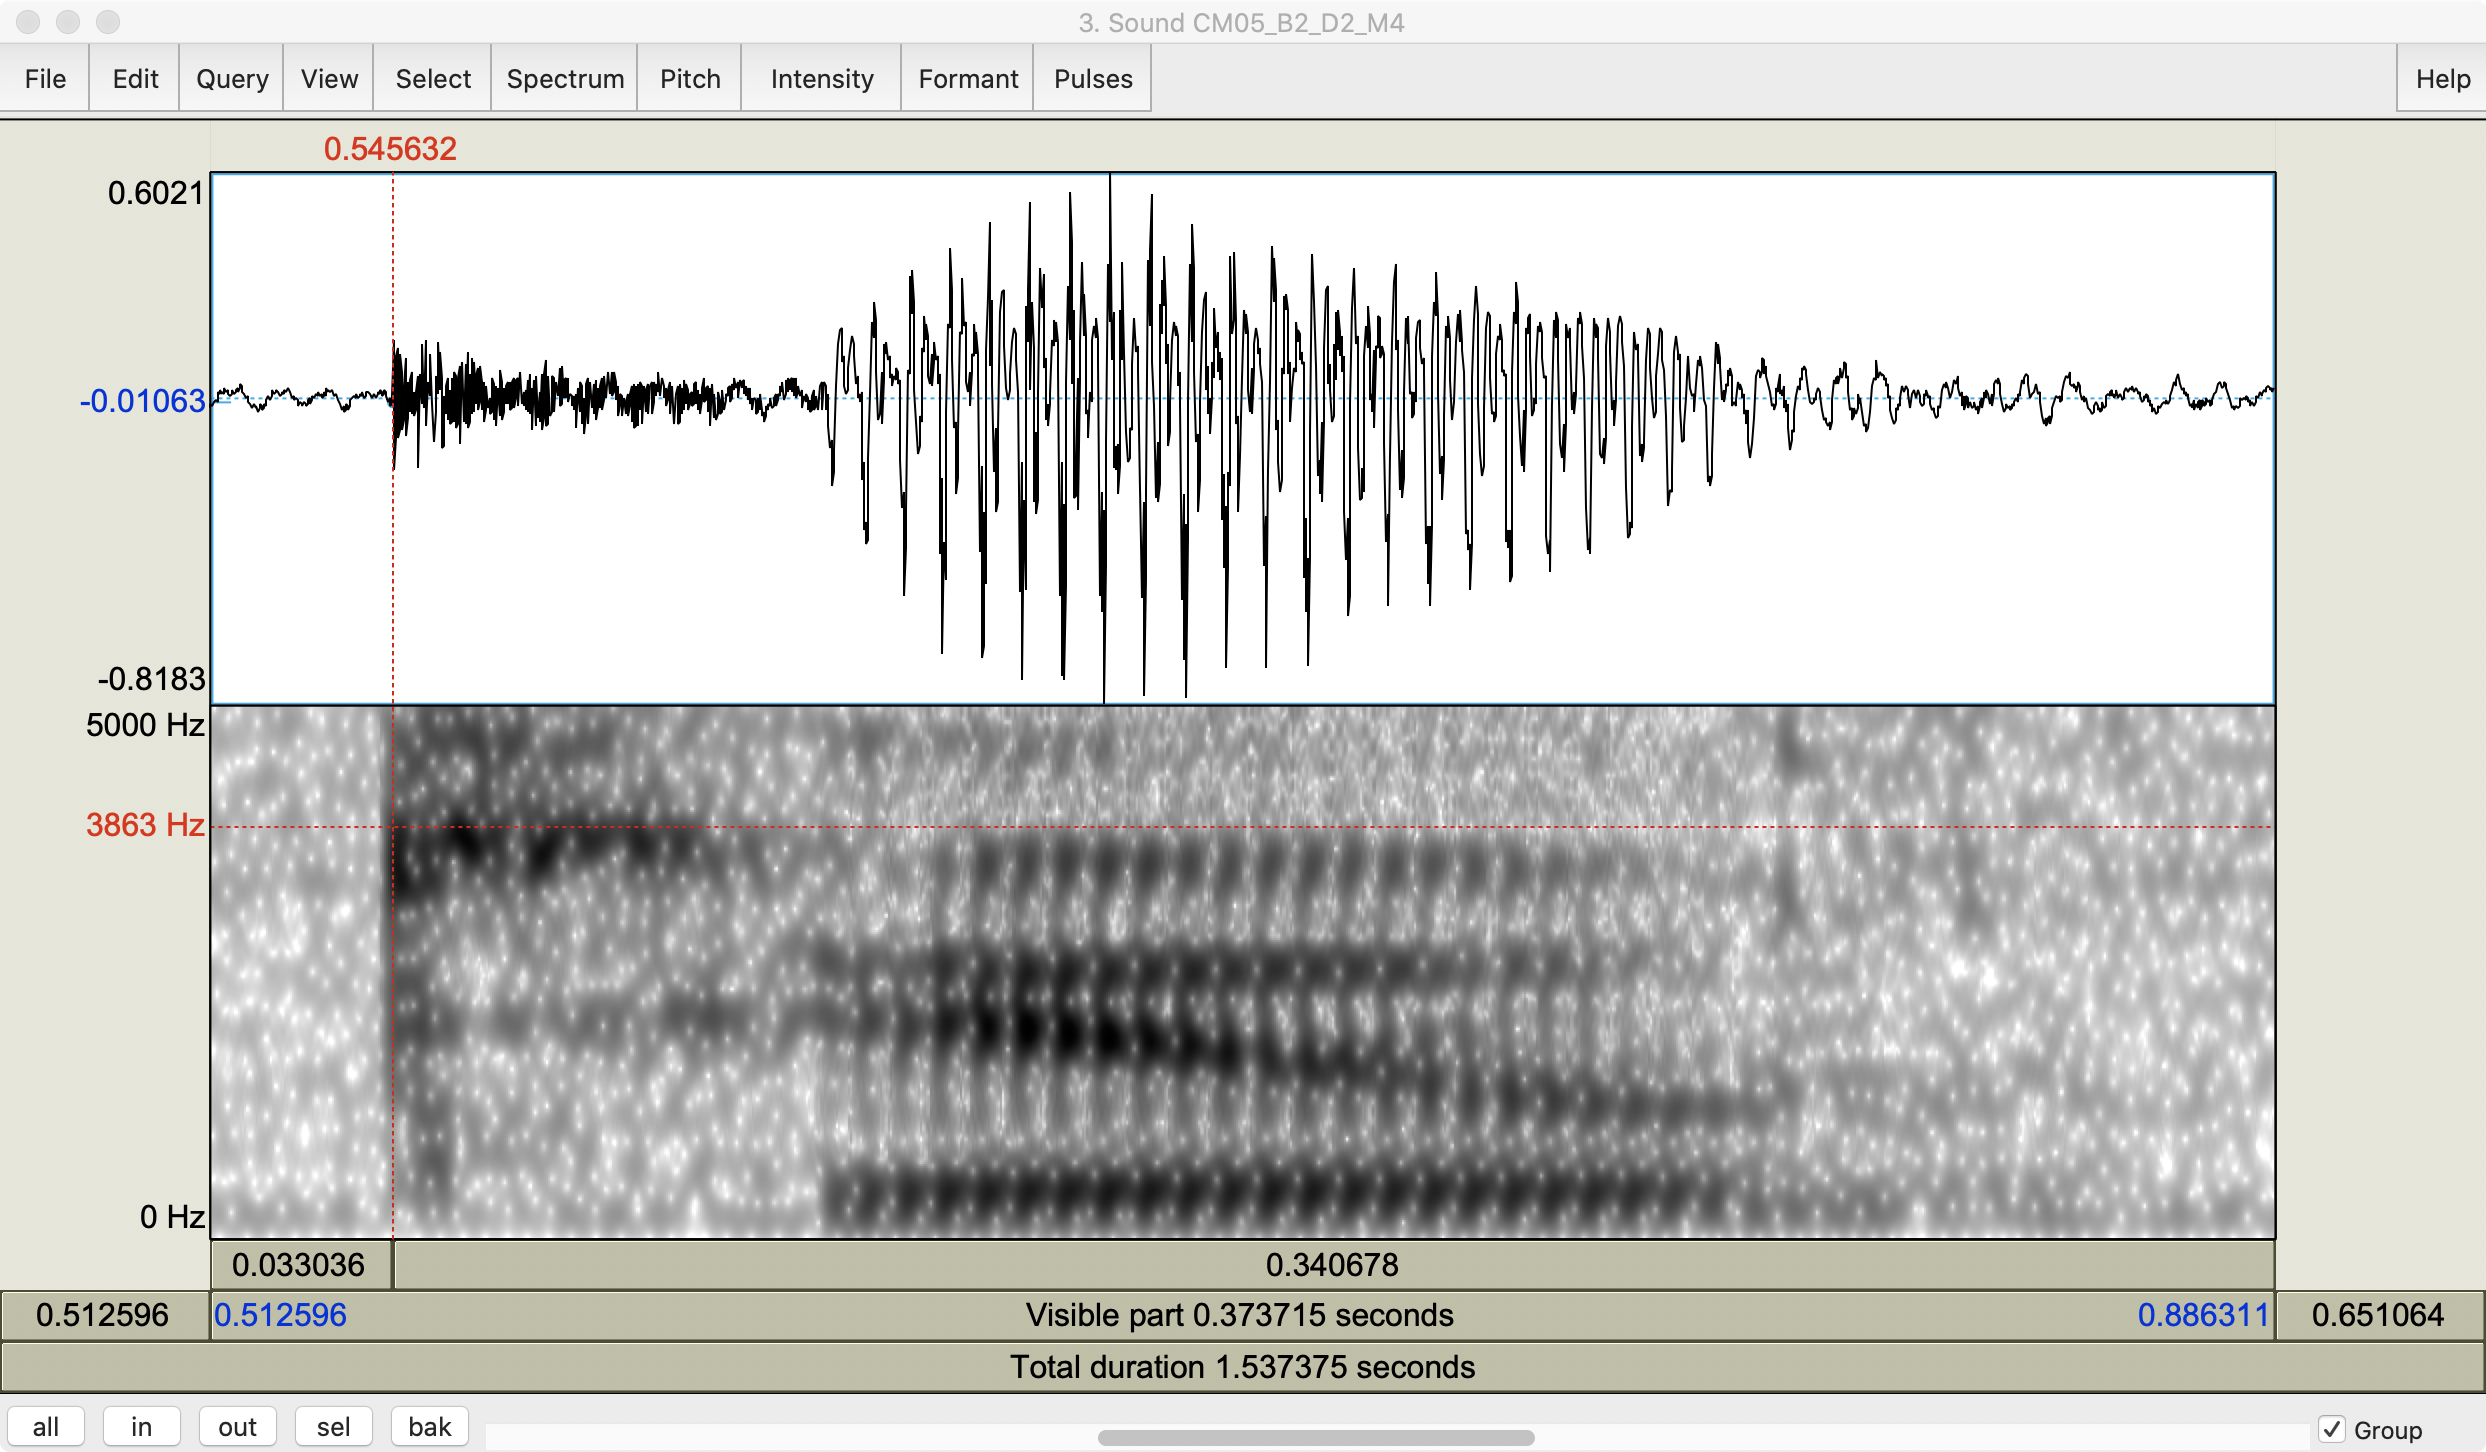
\includegraphics[height=2.5in]{CM05_B2_D2_M4.png}}
\end{frame}

\begin{frame}
  \frametitle{Short Time Fourier Transform}


  The short-time Fourier Transform (STFT) is the Fourier transform of
  a short part of the signal.
  We write either $X_m(\omega)$  of $X_m[k]$ to mean:
  \begin{itemize}
  \item The DFT of the short part of the signal that starts at sample $m$,
  \item windowed by a window of length $L\le N$ samples,
  \item evaluated at frequency $\omega=\frac{2\pi k}{N}$.
  \end{itemize}
  The next several slides will go through this procedure in detail,
  then I'll summarize.
\end{frame}

\begin{frame}
  \frametitle{Step \#1: Chop out part of the signal}

  First, we just chop out the part of the signal starting at sample
  $m$.  Here are examples from Librivox readings of {\em White Fang}
  and {\em Pride and Prejudice}:
  \centerline{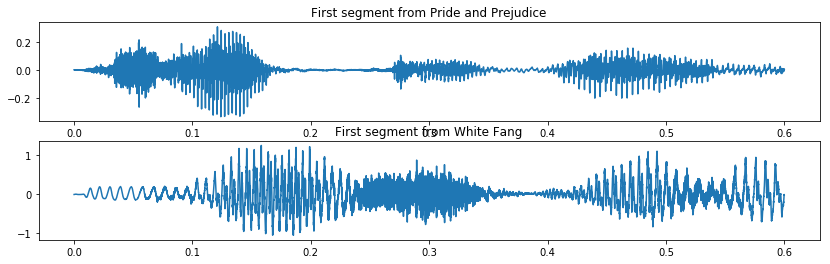
\includegraphics[height=1.5in]{librivox_waves.png}}
\end{frame}

\begin{frame}
  \frametitle{Step \#2: Window the signal}

  Second, we window the signal.  A window with good spectral
  properties is the Hamming window.  The length of the window might be
  $L$, which might be less than the FFT length $N$:
  \[
  w[n] = \begin{cases}
    0.54 - 0.46\cos\left(\frac{2\pi n}{L-1}\right) & 0\le n\le L-1\\
    0 & \mbox{otherwise}
    \end{cases}
  \]
  \centerline{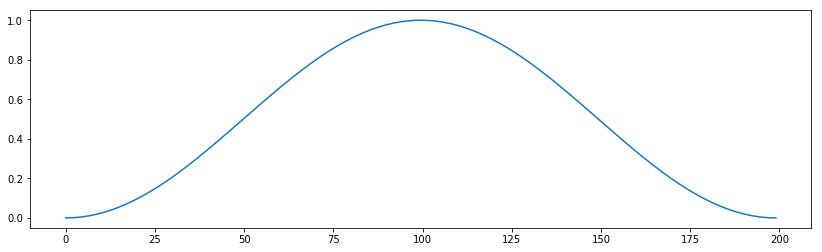
\includegraphics[height=1.25in]{hamming.png}}
\end{frame}

\begin{frame}
  \frametitle{Step \#2: Window the signal}

  Here is the windowed signals, which is nonzero for $0\le n-m\le (L-1)$:
  \[
  x[n,m] = w[n-m]x[n]
  \]
  \centerline{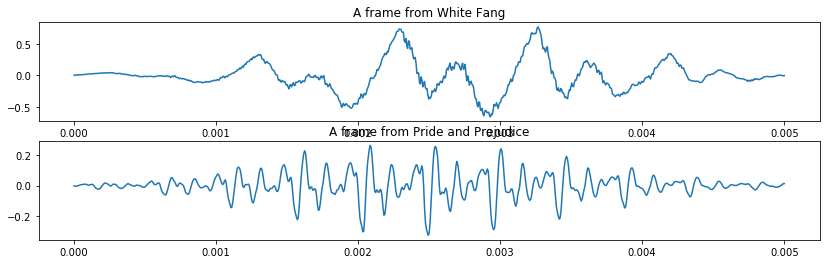
\includegraphics[height=1.5in]{librivox_windowed.png}}
\end{frame}

\begin{frame}
  \frametitle{Step \#3: Fourier Transform}

  Finally, we take the DTFT of the windowed signal.  The result is the
  STFT, $X_m(\omega)$:
  \[
  X_m(\omega) = \sum_{n=m}^{m+(L-1)} w[n-m]x[n]e^{-j\omega (n-m)} 
  \]
  Here it is, plotted as a function of $k$:
  \centerline{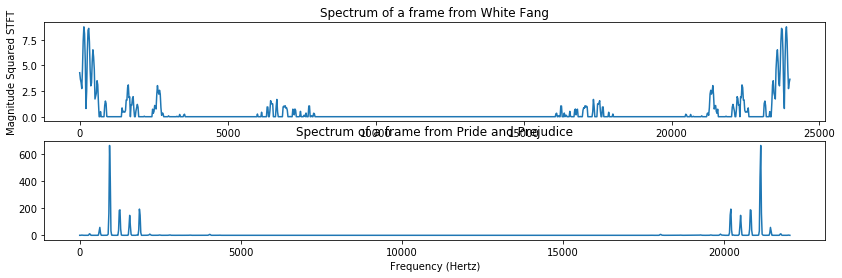
\includegraphics[height=1.5in]{librivox_dftsquared.png}}
\end{frame}

\begin{frame}
  \frametitle{Spectrogram = $20\log_{10}|\mbox{Short Time Fourier Transform}|$}

  \[
  20\log_{10}|X_m(\omega)| = 20\log_{10}\left|\sum_{n}w[n-m]x[n]e^{-j\omega (n-m)}\right|
  \]
  Here it is, plotted as an image, with $k=$row index, $m=$column index.
  \centerline{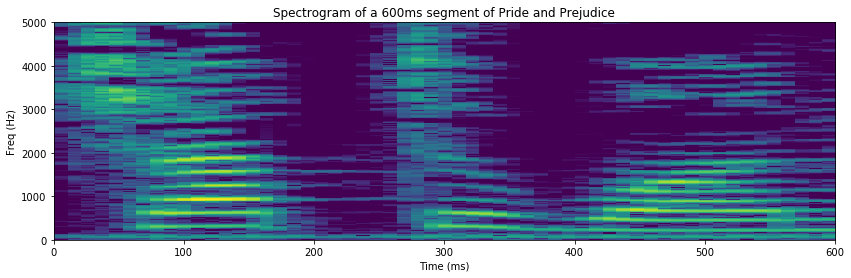
\includegraphics[height=1.5in]{librivox_spectrograms.png}}
\end{frame}

\begin{frame}
  \frametitle{Putting it all together: STFT}
  The STFT, then, is defined as
  \[
  X_m(\omega)= \sum_{n} w[n-m]x[n]e^{-j\omega (n-m)},~~~\omega=\frac{2\pi k}{N}
  \]
  which we can also write as
  \[
  X_m[k] = \mbox{DFT}\left\{w[n]x[n+m]\right\}
  \]
\end{frame}

%%%%%%%%%%%%%%%%%%%%%%%%%%%%%%%%%%%%%%%%%%%%
\section[Linear Frequency]{STFT as a Linear-Frequency Filterbank}
\setcounter{subsection}{1}

\begin{frame}
  \frametitle{STFT as a bank of analysis filters}

  The STFT is defined as:
  \[
  X_m[k] = \sum_{n=m}^{m+(L-1)} w[n-m]x[n]e^{-j\omega_k(n-m)}
  \]
  which we can also write as
  \[
  X_m[k] = x[m] \ast h_k[m]
  \]
  where
  \[
  h_k[m] = w[-m]e^{j\omega_k m}
  \]
  The frequency response of this filter is just the DTFT of $w[-m]$,
  which is $W(-\omega)$, shifted up to $\omega_k$:
  \[
  H_k(\omega) = W\left(\omega_k-\omega\right)
  \]
\end{frame}

\begin{frame}
  \frametitle{Hamming window spectrum}

  The frequency response of this filter is just the DTFT of $w[-m]$,
  which is $W(-\omega)$, shifted up to $\omega_k$:
  \[
  H_k(\omega) = W\left(\omega_k-\omega\right)
  \]
  For a Hamming window, $w[n]$ is on the left, $W(\omega)$ is on the right:
  \centerline{\includegraphics[height=2in]{exp/Hamming.png}}
  \begin{tiny}
    By Olli Niemitalo, public domain image,
    \url{https://en.wikipedia.org/wiki/Window_function}
  \end{tiny}
\end{frame}
  
\begin{frame}
  \frametitle{STFT as a bank of analysis filters}

  So the STFT is just like filtering $x[n]$ through a bank of analysis
  filters, in which the $k^{\textrm{th}}$ filter is a bandpass filter
  centered at $\omega_k$:
  \centerline{\includegraphics[height=2in]{exp/Multidimensional_Analysis_Filter_Banks.jpg}}
  \begin{tiny}
    By Ventetpluie, GFDL,
    \url{https://en.wikipedia.org/wiki/File:Multidimensional_Analysis_Filter_Banks.jpg}
  \end{tiny}
\end{frame}

\begin{frame}
  \frametitle{Short-Time Fourier Transform}
  \begin{itemize}
  \item {\bf STFT as a Transform:}
    \[
    X_m[k] = \mbox{DFT}\left\{w[n]x[n+m]\right\}
    \]
  \item {\bf STFT as a Filterbank:}
    \[
    X_m[k] = x[m] \ast h_k[m],~~~~h_k[m] = w[-m]e^{j\omega_k m}
    \]
  \end{itemize}
\end{frame}


%%%%%%%%%%%%%%%%%%%%%%%%%%%%%%%%%%%%%%%%%%%%
\section{Inverse STFT}
\setcounter{subsection}{1}

\begin{frame}
  \frametitle{Short-Time Fourier Transform}
  \begin{itemize}
  \item {\bf STFT as a Transform:}
    \[
    X_m[k] = \mbox{DFT}\left\{w[n]x[n+m]\right\}
    \]
  \item {\bf STFT as a Filterbank:}
    \[
    X_m[k] = x[m] \ast h_k[m],~~~~h_k[m] = w[-m]e^{j\omega_k m}
    \]
  \end{itemize}
\end{frame}

\begin{frame}
  \frametitle{The inverse STFT}
  STFT as a transform is defined as:
  \[
  X_m[k]= \sum_{n=m}^{m+(N-1)} w[n-m]x[n]e^{-j2\pi k(n-m)/N}
  \]
  Obviously, we can inverse transform as:
  \[
  x[n] = \frac{1}{N w[n-m]}\sum_{k=0}^{N-1} X_m[k]e^{j2\pi k(n-m)/N}
  \]
\end{frame}
\begin{frame}
  \frametitle{The inverse STFT}

  We get a better estimate of $x[n]$ if we average over all of the
  windows for which $w[n-m]\ne 0$.  This is often called the
  overlap-add method, because we overlap the inverse-transformed
  windows, and add them together:
  \[
  x[n] = \frac{\sum_m\frac{1}{N}\sum_{k=0}^{N-1} X_m[k]e^{j\omega_k (n-m)}}{\sum_mw[n-m]}
  \]
  Often, the denominator is a constant, independent of $n$.  That
  happens automatically if there has been no downsampling; it is
  \[
  W(0)=\sum_{m=0}^{N-1} w[m]
  \]
\end{frame}

\begin{frame}
  \frametitle{STFT: Forward and Inverse}
  \begin{itemize}
  \item {\bf Short Time Fourier Transform (STFT)}:
    \[
    X_m[k]= \sum_n w[n-m]x[n]e^{-j\omega_k (n-m)},~~~\omega_k=\frac{2\pi k}{N}
    \]
  \item {\bf Inverse Short Time Fourier Transform (ISTFT, OLA method)}:
    \[
    x[n] = \frac{1}{NW(0)}\sum_m\sum_{k=0}^{N-1} X_m[k]e^{j\omega_k (n-m)}
    \]
  \end{itemize}
\end{frame}

\begin{frame}
  \frametitle{ISTFT as a bank of synthesis filters}

  {\bf Inverse Short Time Fourier Transform (ISTFT)}:
  \[
  x[n] = \frac{1}{NW(0)}\sum_m\sum_{k=0}^{N-1} X_m[k]e^{j\omega_k (n-m)}
  \]
  The ISTFT is the sum of filters:
  \begin{align*}
    x[n] &= \frac{1}{W(0)}\sum_m\sum_{k=0}^{N-1} X_m[k]e^{j\omega_k (n-m)}\\
    &= \sum_{k=0}^{N-1} \left( X_m[k] \ast g_k[m]\right)
  \end{align*}
  where
  \[
  g_k[m] = \begin{cases}
    \frac{1}{W(0)}e^{j\omega_k m} & 0\le m\le N-1\\
    0 & \mbox{otherwise}
  \end{cases}
  \]
\end{frame}

\begin{frame}
  \frametitle{ISTFT as a bank of synthesis filters}

  So the ISTFT is just like filtering $X_m[k]$ through a bank of synthesis
  filters, in which the $k^{\textrm{th}}$ filter is a bandpass filter
  centered at $\omega_k$:
  \centerline{\includegraphics[height=2in]{exp/Multidimensional_Synthesis_Filter_Banks.jpg}}
  \begin{tiny}
    By Ventetpluie, GFDL,
    \url{https://en.wikipedia.org/wiki/File:Multidimensional_Synthesis_Filter_Banks.jpg}
  \end{tiny}
\end{frame}
  
\begin{frame}
  \frametitle{The whole process: STFT and ISTFT as a filterbanks}

  We can compute the STFT, downsample, do stuff to it, upsample, and then resynthesize the
  resulting waveform:
  \centerline{\includegraphics[height=2in]{exp/Multidimensional_M_channel_Filter_Banks.jpg}}
  \begin{tiny}
    By Ventetpluie, GFDL,
    \url{https://en.wikipedia.org/wiki/File:Multidimensional_M_Channel_Filter_Banks.jpg}
  \end{tiny}
\end{frame}
  
%%%%%%%%%%%%%%%%%%%%%%%%%%%%%%%%%%%%%%%%%%%%
\section[Nonlinear Frequency]{Implementing Nonlinear-Frequency Filterbanks Using the STFT}
\setcounter{subsection}{1}

\begin{frame}
  \frametitle{Short-Time Fourier Transform}
  \begin{itemize}
  \item {\bf STFT as a Transform:}
    \[
    X_m[k] = \mbox{DFT}\left\{w[n]x[n+m]\right\}
    \]
  \item {\bf STFT as a Filterbank:}
    \[
    X_m[k] = x[m] \ast h_k[m],~~~~h_k[m] = w[-m]e^{j\omega_k m}
    \]
  \end{itemize}
\end{frame}

\begin{frame}
  \frametitle{Relative Benefits of Transforms vs. Filters}
  \begin{itemize}
  \item {\bf STFT as a Transform:} Implement using Fast Fourier Transform.
    \begin{align*}
      X_m[k]&= \mbox{DFT}\left\{w[n]x[n+m]\right\}\\
      \mbox{\bf Computational Complexity} &= {\mathcal O}\left\{N\log_2(N)\right\}~\mbox{per}~m\\
      \mbox{\bf Example:} & N=1024\\
      \mbox{\bf Computational Complexity} &= 10240~\mbox{multiplies/sample}
    \end{align*}
  \item {\bf STFT as a Filterbank:} Implement using convolution.
    \begin{align*}
      X_m[k]&= x[m]\ast h_k[m]\\
      \mbox{\bf Computational Complexity} &= {\mathcal O}\left\{N^2\right\}~\mbox{per}~m\\
      \mbox{\bf Example:} & N=1024\\
      \mbox{\bf Computational Complexity} &= 1048576~\mbox{multiplies/sample}
    \end{align*}
  \end{itemize}
\end{frame}

\begin{frame}
  \frametitle{What about other filters?}

  \begin{itemize}
  \item Obviously, FFT is much faster than the convolution approach.
  \item Can we use the FFT to speed up other types of filter computations, as well?
  \item For example, can we model the bandpass filtering operations of the human ear
    from the STFT?
  \end{itemize}
\end{frame}

\begin{frame}
  \frametitle{What about other filters?}

  \begin{itemize}
    \item 
      We want to find $y[n]=f[n]\ast x[n]$, where
      $f[n]$ is a length-$N$ impulse response.
    \item Complexity of the convolution in time domain is
      ${\mathcal{O}}\left\{N\right\}$ per output sample.
    \item We can't find $y[n]$ exactly, but we can find
      $\tilde{y}[n]=f[n]\circledast (w[n-m]x[n])$ from the STFT:
      \[
      Y_m[k] = F[k]X_m[k]
      \]
    \item It makes sense to do this only if $F[k]$ has far fewer than
      $N$ non-zero terms (narrowband filter).
  \end{itemize}
\end{frame}

\begin{frame}
  \frametitle{Bandpass-Filtered Signal Power}

  In particular, suppose that $f[n]$ is a bandpass filter, and we'd
  like to know how much power gets through it.

  So we'd like to know the power of the signal
  $\tilde{y}[n]=f[n]\circledast (w[n-m]x[n])$.  We can get that as
  \begin{align*}
    \sum_{n=0}^{N-1} \tilde{y}[n]^2 
    &= \frac{1}{N}\sum_{k=0}^{N-1} |Y_m[k]|^2\\
    &= \frac{1}{N}\sum_{k=0}^{N-1} |F[k]|^2 |X_m[k]|^2
  \end{align*}
\end{frame}

%%%%%%%%%%%%%%%%%%%%%%%%%%%%%%%%%%%%%%%%%%%%
\section[Summary]{Summary}
\setcounter{subsection}{1}

\begin{frame}
  \frametitle{Summary}
  \begin{itemize}
  \item {\bf STFT as a Transform:}
    \[
    X_m(\omega)= \sum_n w[n-m]x[n]e^{-j\omega (n-m)},~~~\omega_k=\frac{2\pi k}{N}
    \]
  \item {\bf STFT as a Filterbank:}
    \[
    X_m(\omega) = x[m] \ast h_k[m],~~~~h_\omega[m] = w[-m]e^{j\omega m}
    \]
  \item {\bf Other filters using STFT:}
    \[
    \mbox{DFT}\left\{f[n] \circledast (w[n-m]x[n])\right\} = H[k]X_m[k]
    \]
  \item {\bf Bandpass-Filtered Signal Power}
    \[
    \sum_{n=0}^{N-1} \tilde{y}[n]^2 
    = \frac{1}{N}\sum_{k=0}^{N-1} |F[k]|^2 |X_m[k]|^2
    \]
  \end{itemize}
\end{frame}  

\end{document}

